\subsection*{Monte Carlo Sampling}

% Week 8

\begin{defe}[Empirical distribution] \label{defe: em_dist}
    Let $x_1 , \ldots , x_n$ be an iid real-valued sample from a cdf $F$. The function
    \begin{equation*}
        F_{n} (x) = \frac{1}{N} \sum_{i=1}^{N} \Id_{\left\{ x_i \leq x \right\}} (x) , \quad x \in \RR
    \end{equation*}
    is called the {\bf empirical cdf} of the data \cite{KroeseDirkP2013SMaC}*{page 196}.
\end{defe}

\begin{figure}[ht]
    \centering
    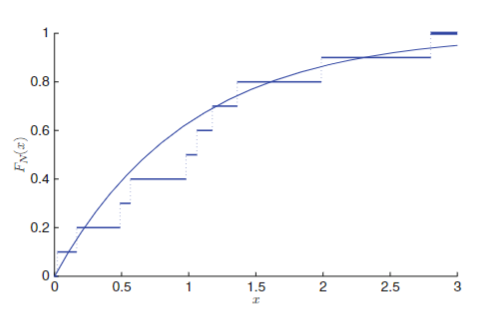
\includegraphics[scale=1.0]{img/bay_inf/emp_cdf_exp_1.png}
    \caption{The empirical cdf \ref{defe: em_dist} for a sample size $10$ from a $\Exp (0.2)$ distribution as well as the true cdf. Image from \cite{KroeseDirkP2013SMaC}*{page 197}.}
    \label{fig: emp_cdf_exp_1}
\end{figure}

Note that for the ordered sample $x_{(1)} < x_{(2)} < \cdots < x_{(N)}$,

\begin{equation*}
    F_{N} \left( x_{(i)} \right) = \frac{i}{N}.
\end{equation*}

assuming for the sake of simplicity that all $\left\{ x_i \right\}$ take on different values. If instead of deterministic $\left\{ x_i \right\}$ we take random $X_i$, then $F_N (x)$ becomes random as well. To distinguish between the deterministic and the random case, let us denote the random empirical cdf by $\hat{F}_{N} (x)$. We now have
\begin{equation*}
    \PP \left[ \hat{F}_{N} (x) = \frac{i}{N} \right] = \PP \left[ X_{(i)} \leq x , X_{(i+1)}  x \right] = \binom{N}{i} \left( F(x) \right)^{i} \left( 1 - F(x) \right)^{N-i}
\end{equation*}
\cite{KroeseDirkP2013SMaC}*{page 198}. The above equation can be summarized as $N \hat{F}_{N} (x) \sim \Bin (N, F(x))$. Consequently,
\begin{align*}
    \EE \left[ \hat{F}_{N} (x) \right]  & = F(x)                          \\
    \Var \left[ \hat{F}_{N} (x) \right] & = F(x) \left( 1 - F(x) \right).
\end{align*}
Moreover, by the law of large numbers and the central limit theorem, we have
\begin{equation*}
    \PP \left[ \lim_{N \to \infty} \hat{F}_{N} (x) = F (x) \right] = 1,
\end{equation*}
and
\begin{equation*}
    \lim_{N \to \infty} \PP \left[ \frac{\hat{F}_{N} (x) - F(x)}{\sqrt{F(x)(1-F(x)/N)}} \right] = \Phi (z).
\end{equation*}

\begin{defe}[Confidence Intervals] \label{defe: confd_int}
    Let $X_1 , \ldots , X_n$ be random variables with a joint distribution depdending on a parameter $\theta \in \Theta$. Let $T_1 < T_2$ be functions of the data but not of $\theta$. The random interval $(T_1 , T_2)$ is called a {\bf stochastic confidence interval} for $\theta$ with confidence $1 - \alpha$ if
    \begin{equation*}
        \PP_{\theta} \left[ T_1 < \theta < T_2 \right] \geq 1 - \alpha \quad \text{for all} \quad \theta \in \Theta.
    \end{equation*}
    If $t_1$ and $t_2$ are the observed values of $T_1$ and $T_2$, then the interval $(t_1 , t_2)$ is called the {\bf numerical confidence interval} for $\theta$ with confidence $1 - \alpha$ \cite{KroeseDirkP2013SMaC}*{page 128}.
\end{defe}

An approximate $1 - \alpha$ confidence interval for $F(x)$ is
\begin{equation*}
    F_N (x) \pm z_{1 - \alpha / 2} \sqrt{\frac{F_N (x) (1 - F_N (x))}{N}}
\end{equation*}
where $z_{1 - \alpha / 2}$ is the $1 - \alpha / 2$ quantile of the standard normal distribution. Moreover for the ordered sample $x_{(1)} < x_{(2)} < \cdots < x_{(N)}$, an approximate $1 - \alpha$ confidence interval for $F(x_{(i)})$ is
\begin{equation*}
    \frac{i}{N} \pm z_{1 - \alpha / 2} \sqrt{\frac{i(1 - i/n)}{N^2}}
\end{equation*}
\cite{KroeseDirkP2013SMaC}*{page 198}.

\subsubsection*{Simultaneous Confidence Bands}

% Week Lec 2, Ch 7.1

\begin{defe}[Kolmogorov–Smirnov statistic] \label{defe: TBD}
    For a continuous $F$, the statistic of
    \begin{equation*}
        D_n = \sup_{x \in \RR} \left| \hat{F}_N (x) - F(x) \right|
    \end{equation*}
    is called the {\bf Kolmogorov–Smirnov statistic} \cite{KroeseDirkP2013SMaC}*{page 200}.
\end{defe}

Note that this statistic does not depend on $F$ and can be used to test whether iid samples $X_1 , \ldots , X_n$ come from a specified distribution as well as constructing a simultaneous confidence band for $F$. The empirical cdf can be used to estimate any cdf, both discrete and continuous, but it is always 'jumpy' which may be undesirable, for example when the underlying distribution is continuous. When we have continuous data, we may want a continuous density estimate instead. This leads to our next topic of density estimation.

\subsubsection*{Kernel Density Estimation}

\begin{defe}[Kernel Density Estimator] \label{defe: KDE}
    Let $X_1 , \ldots X_n \iid f$ from a continuous distribution with cdf $F$. A {\bf Kernel density estimator} (KDE), also known as a sliding window estimator, with bandwidth $h$ is given by
    \begin{equation*}
        \hat{f} (x;h) = \frac{1}{N} \sum_{i=1}^{N} K \left( \frac{x_i - x}{h} \right).
    \end{equation*}
    The function $K (\cdot)$ is the kernel function ("window shape") and $h$ is the window ("window size").
\end{defe}

There are many choice of $K$, but we shall just focus on the Gaussian kernel.

\begin{defe}[Gaussian Kernel] \label{defe: gauss_kern}
    The {\bf Gaussian Kernel} uses a kernel of
    \begin{equation*}
        K(x) = \frac{1}{\sqrt{2 \pi}} \exp \left( - \frac{1}{2} x^2 \right)
    \end{equation*}
    so that
    \begin{equation*}
        \hat{f} (x;h) = \frac{1}{N} \sum_{i=1}^{N} \frac{1}{\sqrt{2 \pi}} \exp \left( - \frac{1}{2} \left( \frac{x_i - x}{h} \right)^2 \right)
    \end{equation*}
    \cite{KroeseDirkP2013SMaC}*{page 201}.
\end{defe}

Essentially, the Gaussian kernel is just an equally weighted $\frac{1}{N}$ normal mixture model. It has $N$ Gaussian "humps", centered at each observation and has standard deviation $h$. As it turns out, the choice of the kernel is not that crucial, but the choice of the bandwidth is very important.